\documentclass[]{article}
\usepackage{lmodern}
\usepackage{amssymb,amsmath}
\usepackage{ifxetex,ifluatex}
\usepackage{fixltx2e} % provides \textsubscript
\ifnum 0\ifxetex 1\fi\ifluatex 1\fi=0 % if pdftex
  \usepackage[T1]{fontenc}
  \usepackage[utf8]{inputenc}
\else % if luatex or xelatex
  \ifxetex
    \usepackage{mathspec}
  \else
    \usepackage{fontspec}
  \fi
  \defaultfontfeatures{Ligatures=TeX,Scale=MatchLowercase}
\fi
% use upquote if available, for straight quotes in verbatim environments
\IfFileExists{upquote.sty}{\usepackage{upquote}}{}
% use microtype if available
\IfFileExists{microtype.sty}{%
\usepackage{microtype}
\UseMicrotypeSet[protrusion]{basicmath} % disable protrusion for tt fonts
}{}
\usepackage[margin=1in]{geometry}
\usepackage{hyperref}
\hypersetup{unicode=true,
            pdftitle={The value of information to the risk-averse conservation decision maker},
            pdfauthor={William K Morris},
            pdfborder={0 0 0},
            breaklinks=true}
\urlstyle{same}  % don't use monospace font for urls
\usepackage{natbib}
\bibliographystyle{voiRisk.bst}
\usepackage{longtable,booktabs}
\usepackage{graphicx,grffile}
\makeatletter
\def\maxwidth{\ifdim\Gin@nat@width>\linewidth\linewidth\else\Gin@nat@width\fi}
\def\maxheight{\ifdim\Gin@nat@height>\textheight\textheight\else\Gin@nat@height\fi}
\makeatother
% Scale images if necessary, so that they will not overflow the page
% margins by default, and it is still possible to overwrite the defaults
% using explicit options in \includegraphics[width, height, ...]{}
\setkeys{Gin}{width=\maxwidth,height=\maxheight,keepaspectratio}
\IfFileExists{parskip.sty}{%
\usepackage{parskip}
}{% else
\setlength{\parindent}{0pt}
\setlength{\parskip}{6pt plus 2pt minus 1pt}
}
\setlength{\emergencystretch}{3em}  % prevent overfull lines
\providecommand{\tightlist}{%
  \setlength{\itemsep}{0pt}\setlength{\parskip}{0pt}}
\setcounter{secnumdepth}{5}

%%% Use protect on footnotes to avoid problems with footnotes in titles
\let\rmarkdownfootnote\footnote%
\def\footnote{\protect\rmarkdownfootnote}

%%% Change title format to be more compact
\usepackage{titling}

% Create subtitle command for use in maketitle
\newcommand{\subtitle}[1]{
  \posttitle{
    \begin{center}\large#1\end{center}
    }
}

\setlength{\droptitle}{-2em}
  \title{The value of information to the risk-averse conservation decision maker}
  \pretitle{\vspace{\droptitle}\centering\huge}
  \posttitle{\par}
  \author{William K Morris}
  \preauthor{\centering\large\emph}
  \postauthor{\par}
  \predate{\centering\large\emph}
  \postdate{\par}
  \date{2017-09-19}

\usepackage{titlesec}
\titleformat{\paragraph}{\small\normalfont\bfseries}{}{0pt}{}
\titleformat{\subparagraph}{\small\normalfont}{}{0pt}{}
\linespread{2}\selectfont
\usepackage{booktabs}
\usepackage{setspace}
\usepackage{caption}
\usepackage{tikz}
\usepackage{pdflscape}
\captionsetup{font={stretch=2}}
\usepackage{pbox}
\usepackage[displaymath,mathlines]{lineno}
\linenumbers

\usepackage{amsthm}
\newtheorem{theorem}{Theorem}[section]
\newtheorem{lemma}{Lemma}[section]
\theoremstyle{definition}
\newtheorem{definition}{Definition}[section]
\newtheorem{corollary}{Corollary}[section]
\newtheorem{proposition}{Proposition}[section]
\theoremstyle{definition}
\newtheorem{example}{Example}[section]
\theoremstyle{definition}
\newtheorem{exercise}{Exercise}[section]
\theoremstyle{remark}
\newtheorem*{remark}{Remark}
\newtheorem*{solution}{Solution}
\begin{document}
\maketitle


\subsection*{Abstract}\label{abstract}
\addcontentsline{toc}{subsection}{Abstract}

Conservation and natural resource management has begun to incorporate value of information analyses into its arsenal of decision making tools. To date however, these analytical techniques have only been explored from a risk-neutral standpoint. Risk profile affects the value of information. Here, with a simple illustrative example, we demonstrate how different decision makers with different risk tolerances would value information. Intuitively one might assume that a risk-averse decision maker would always prefer to learn before making a decision. But as the example here demonstrates, this will not always be the case. Sometimes new information is less valuable to a risk-averse decision maker than it is to other, more risk-tolerant, decision makers. This is important because it highlights that not only is it important to identify critical uncertainties for decision making it is important to identify them in the context of risk-tolerence and not simply assume that risk-aversion increases information value.

\subsection*{Introduction}\label{introduction}
\addcontentsline{toc}{subsection}{Introduction}

Information matters to conservation decision makers because it can help
them make better decisions \citep{Canessa2015}. But new information is
not uniformly important to all decisions, it matters more to some
decisions than others, and its potential contribution can be assessed
through value of information analyses \citep{Yokota2004b}. Such
decisions can also be sensitive to the decision maker's attitude to
risk, depending on how conservative or aspirational they are
\citep{Burgman2005}. Hence, it can be expected that risk profile matters
when considering the value of information \citep{Eeckhoudt2000}.

Examples of valuing information for conservation and natural resource
management to date consider expected value of information
\citep[e.g.,][]{Moore2011, Runge2011, Johnson2014a, Canessa2015, Maxwell2015}.
That is, the value of information from the perspective of a risk-neutral
decision maker. Often, risk neutrality may not be an appropriate
assumption. Risk aversion is a perhaps the more common stance among many
conservation decision makers \citep{Tulloch2015}. This is highlighted in
particular by espousing and applying the precautionary principle
\citep{Johnson2012, Falcy2016}. Intuitively, it might seem that risk
aversion would lead to a higher value of information, as ``having the
facts'' first would be perceived as an inherently less risky decision
making strategy. However, risk aversion does not automatically increase
the value of information. Depending on the situation, it can even
decrease the value of information \citep{Gould1974}. We illustrate with
the example below.

The following presents an adaptation of the ``newsboy problem'', a
simple case-study used in applied statistics, decision theory and
economics for over a century \citep{Edgeworth1888}.
\citet{Eeckhoudt2000} first used this model to illustrate the role of
risk in information valuing, building on the work of \citet{Gould1974}
and \citet{Willinger1989}. However, none of these works have so far had
an impact on the conservation sciences, so we present the current work
in attempt to package their ideas in a form appropriate for a
conservation and natural resource management audience. The implication
of the present work is that risk and information value have a more
complex relationship than one might gather from the conservation and
natural resource management value of information work presented to date.

\subsection*{Conservation manager's
dilemma}\label{conservation-managers-dilemma}
\addcontentsline{toc}{subsection}{Conservation manager's dilemma}

A conservation manager is tasked with managing a population of animals.
At present the population consists of 10 breeding pairs and is at it's
carrying capacity. However, an invasive plant is degrading the habitat
of the population and by the next year will reduce the breeding
population to 8 pairs. The manager has the option to restore the invaded
part of the habitat. But, the outcome of any restoration effort is
uncertain. If successful, the carrying capacity will increase beyond the
current level to 15 breeding pairs. There is some probability, \(p\),
that the restoration efforts will fail to increase the amount of
suitable habitat, as in the past, not all restorations of this kind have
worked. If the restoration fails, it will reduce the carrying capacity
further even than the invasive plant would if left to its own devices,
leaving only 5 breeding pairs. Left with this decision the conservation
manager must consider the payoff matrix below (Table \ref{tab:payoff}).

\clearpage

\begin{longtable}[]{@{}lll@{}}
\caption{\label{tab:payoff} Payoff matrix for conservation manager's
decision. When the ``do nothing'' option is taken, the manager is
guaranteed 8 breeding pairs. When the manager chooses to restore the
invaded habitat there is some probability, \(p\), that the restoration
fails and only 5 breeding pairs remain. On the other hand, if the
restoration succeeds (which has a probability of 1 - \(p\)), the
carrying capacity will rise to 15 breeding pairs.}\tabularnewline
\toprule
\emph{Action} & \(p\) & 1 - \(p\)\tabularnewline
\midrule
\endfirsthead
\toprule
\emph{Action} & \(p\) & 1 - \(p\)\tabularnewline
\midrule
\endhead
Do nothing & 8 & 8\tabularnewline
Restore & 5 & 15\tabularnewline
\bottomrule
\end{longtable}

If the manager is risk-neutral, then the action they should take is the
one that maximizes expected value \citep{Burgman2005}. Fig
\ref{fig:riskev} (top left panel) shows that this value is dependent on
\(p\). When \(p\) is between 1 (a 100\% chance of failure) and 0.7 the
optimal decision is to leave the invasion to proceed. Here 0.7 is the
probability such that,

\begin{equation}
  8p + 8(1 - p) = 5p + 15(1 - p)
  \label{eq:pcrit}
\end{equation}

In other words, this is the probability of failure where the expected
value (the sum of the outcomes multiplied by their probabilities of
happening) of making either decision is the same. With a chance of
failure of 0.7 or higher, which we will call, \(p_\textit{crit}\),
restoration would always have an expected value, \(5p + 15(1 - p)\),
that is less than 8, the expected value of not doing anything, which
should be the managers decision. If the probability of failure decreases
beyond \(p_\textit{crit}\) then the expected value of restoration will
be greater than the do-nothing option, so restoration should be
preferred.
















\begin{figure}[htbp]
\centering
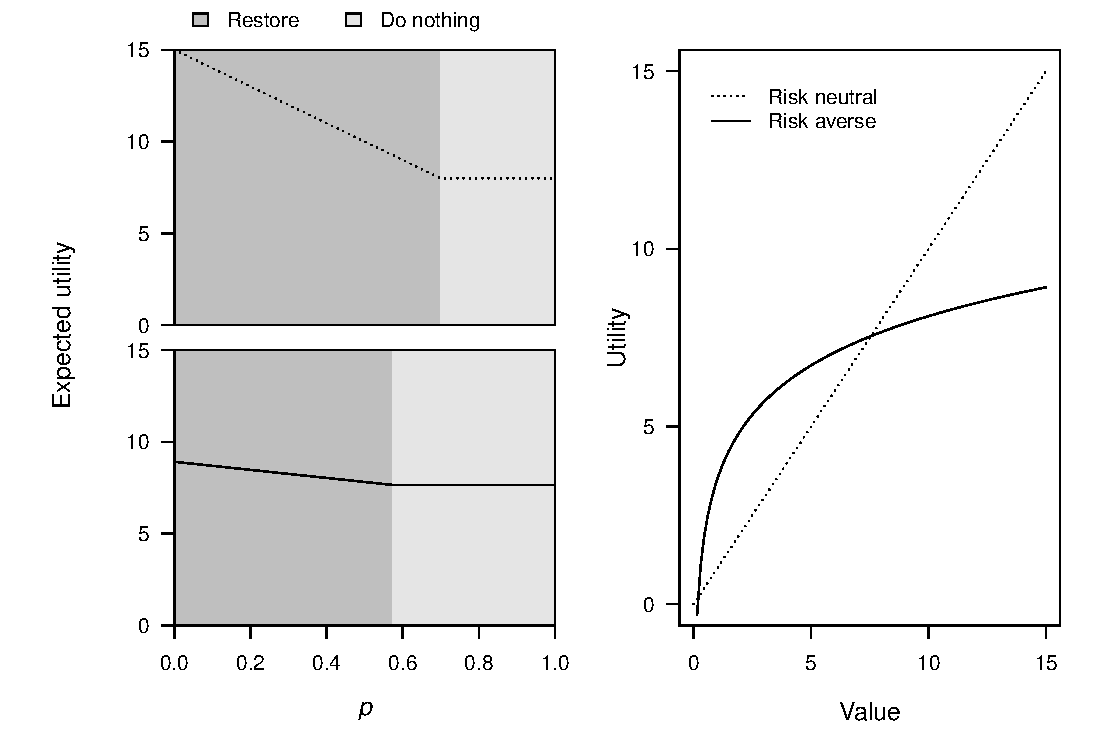
\includegraphics{_main_files/figure-latex/riskev-1.pdf}
\caption{\label{fig:riskev}Risk tolerance and expected utility. Left panels show the
relationship between expected utility and the probability, \(p\), of
restoration failing (black lines). The grey shaded regions indicate the
optimal strategy (restore or do nothing) given \(p\). Top left panel
describes this scenario for a risk-neutral decision maker, while the
panel underneath applies to the point of view of a risk-averse decision
maker. The right panel shows the relative perception of values (utility)
in the payoff matrix (Table \ref{tab:payoff}) for the two different risk
tolerances of the left panels. A risk averse decision maker perceives
the payoff above what can be achieved with a do-nothing strategy, as
having less utility relative to the perception of the risk neutral
decision maker. The effect is to decrease the tolerance to the risk of
restoration failure, moving the value of \(p_\textit{crit}\), the point
at which ``do nothing'' is optimal, to the left.}
\end{figure}

\subsection*{Expected value of
information}\label{expected-value-of-information}
\addcontentsline{toc}{subsection}{Expected value of information}

Now suppose that before making a decision, the manager can find out with
certainty whether or not the restoration will be successful (by testing
the soil for example). The value of this knowledge, for the risk-neutral
decision maker, is the expected value of perfect information (EVPI). The
EVPI is the difference between the expected value under uncertainty (the
line in the top left panel of figure \ref{fig:riskev}) and the expected
value with perfect information (EVWPI). We have already calculated the
expected value under uncertainty (also known as the expected value with
original information, EVWOI) above. The EVWPI also varies with \(p\),
and is calculated by considering what action would be taken under each
circumstance of knowing if restoration would fail or not, and then
multiplying the outcome of each scenario by the probability of success
and failure respectively (i.e., in this case
\(\mathrm{EVPWI} = 8p + 15(1-p)\)).

Figure \ref{fig:eupi} (dashed line) shows the relationship between EVPI
and \(p\). Here we see that EVPI is greatest at the point were the
decision switches from restore to do nothing. This makes intuitive
sense, as information should be most valuable when you are most
uncertain about what to do. On both side of this critical probability,
the EVPI decreases as the manager is more sure of what the outcome of
the decision will be (and so more sure of what choice to make), until
such a point that they are completely certain (\(p = 0\) or \(p = 1\)).
At this point of certainty, the value of information is zero. One way to
interpret the EVPI is as the upper limit on what should be spent on
acquiring any new information to help with decision making. For example,
if the conservation manager knew how much an increase in carrying
capacity of one breeding pair was worth (perhaps based on what they or
other managers had spent to achieve this outcome in the past) then they
could not justify spending more than that amount of money on information
unless \(p\) was between 0.33 and 0.86. As outside this range the EVPI
is less than one breeding pair.

\subsection*{Risk-averse decision
making}\label{risk-averse-decision-making}
\addcontentsline{toc}{subsection}{Risk-averse decision making}

Now we will address the same problem from the perspective of a
risk-averse manager. But first we must define what we mean by
risk-aversion. Risk aversion indicates a decision maker's asymmetric
preference for variation in payoff and a propensity to prefer relatively
certain, small returns, to uncertain returns that could be high or low
\citep{Burgman2005}. Risk-neutral decision makers, on the other hand,
are insensitive to this risk, the variation in payoff, and will only
take the expected values of a set of options into account when making a
decision.

As should be clear by now, risk-averse decision makers perceive value
differently to risk-neutralists. To account for this difference,
theorists use the concepts of utility and expected utility in place of
value and expected value. For a risk-neutral decision maker value is
linearly related to utility, but for a risk-averse decision maker the
relationship is concave and diminishing (Figure \ref{fig:riskev} right
panel). Meaning that for the risk-averse, an incremental increase, from
relatively low value to a somewhat higher value, is perceived as a
greater performance increase than incrementing by the same amount up
from an already high value. For example, the right panel of figure
\ref{fig:riskev} indicates that for this risk-averse decision maker,
going from 10 to 15 breeding pairs is perceived as being only about half
the performance increase as going from 0 to 5.

The bottom left panel of figure \ref{fig:riskev} shows the effect of
risk-aversion on the relationship between expected utility (in the risk
neutral case above, value is equivalent to utility) and the probability
of restoration failure. First, across the range of \(p\) where
restoration is the preferred option, the expected utility is reduced, as
even when likely, the potential increase in carrying capacity is
perceived as less important than it is under risk-neutrality. And
second, the range of \(p\) over which restoration is preferred is now
smaller because the critical point where its expected utility is equal
to the do nothing option, is now lower. In effect, the risk-averse
decision maker must be more sure of a positive outcome of restoration to
switch from the sure bet of doing nothing, ensuring a moderate outcome
(8 breeding pairs) and avoiding the possibility of enduring the worst (5
breeding pairs).

\subsection*{Risk aversion and the expected utility of
information}\label{risk-aversion-and-the-expected-utility-of-information}
\addcontentsline{toc}{subsection}{Risk aversion and the expected utility
of information}

As discussed above, to be risk-averse is to have an asymmetric view of
uncertainty. As is shown in figure \ref{fig:riskev} the risk-averse
decision maker prefers to do nothing unless they are more sure, relative
to the risk-neutral decision maker, of restoration success. Therefore,
one might assume that information, which would decrease the uncertainty
in decision making, would be more valuable to the risk-averse decision
maker than to the risk-neutral decision maker. However, as we show
below, this is not always the case and depending on the initial level of
uncertainty the opposite can sometimes be true.

In a previous section we demonstrated how to calculate the EVPI. Now,
after shifting from measuring performance as value, to measuring
performance as utility, we could simply apply the same method to
calculate an expected utility of perfect information (EUPI) instead.
However, calculated in this way, the two quantities, the EUWPI for a
risk-averse decision maker and the EVWPI for a risk-neutral decision
maker, are not on equivalent scales when the relationship between
utility and value is non-linear.

To overcome the non-equivalence of EUWPI and EVWPI due to their
non-linear relationship, we must reformulate them in a slightly
different way. Where before we discussed EVPI as the magnitude of
performance increase moving from uncertainty to certainty, to express
EUPI on the same scale we use an alternative method outline by
\citet{Eeckhoudt2000} and which we show here.

For any given utility function, \(U\) (including the linear function of
risk neutral), the EUPI for the conservation decision at hand can be
defined as,

\begin{equation}
\begin{split}
&\textrm{if}\;\;p \leq p_\textit{crit},\;\;\textrm{then}\;\;pU(8 - \mathrm{EUPI}) + (1 - p)U(15 - \mathrm{EUPI}) = pU(5) + (1 - p)U(15) \\
&\textrm{if}\;\;p \geq p_\textit{crit},\;\;\textrm{then}\;\;pU(8 - \mathrm{EUPI}) + (1 - p)U(15 - \mathrm{EUPI}) = U(8)\\
& \textrm{where}\;\; p_\textit{crit} = \frac{U(8) - U(15)}{U(5) - U(15)}
\label{eq:eupi}
\end{split}
\end{equation}

In other words, the expected utility of getting the best return minus
the maximum cost of learning what action will lead to the best outcome
(which is the EUPI), needs to equal the expected utility of making the
decision without knowing what outcome the actions will lead to (the
expected utility under uncertainty). When \(p \leq p_\textit{crit}\) the
right hand side of this equality is the expected utility of restoration.
Whereas, when \(p \geq p_\textit{crit}\) then the expected utility,
having eliminated uncertainty, must equal the utility of doing nothing.

Figure \ref{fig:eupi} shows the results of solving equation
\eqref{eq:eupi} over the range of \(p\) for the risk neutral and risk
averse utility functions of figure \ref{fig:riskev}. What should be
clear is that assumming that information is always more valuable to the
risk averse is incorrect. For this example, there is a range of \(p\)
where information is more valuable to the risk-averse. When \(p\) is
below or near the point where the risk-averse decision maker would
choose to restore under uncertainty, information is relatively more
important to the risk-averse than it is to the risk-neutral decision
maker. For higher values of \(p\) however, the preferences are reversed
and information is more important to the risk-neutral decision maker
than the risk-averse.

So why would a decision maker that is averse to risk be less willing to
resolve uncertainty than a decision maker who is more tolerant? Before
addressing this, let's first turn to the more intuitive case where
risk-aversion leads to greater utility of information. When the
probability of restoration failure is low, both decision makers take the
gamble that restoration will give them a better expected outcome than
doing nothing. Being sensitive to the uncertainty about the success of
restoration, the risk-averse decision maker is more willing to endure a
certain loss to resolve that uncertainty. They are less satisfied with
the range of outcomes of restoration. However, this state of mind does
not apply when the probability of restoration failure is high. In this
scenario, the decision makers, without extra information, will not take
the gamble and thus prefer the known outcome of doing nothing over the
risk of failing after trying to restore. At this point the gamble now
becomes the act of paying to learn about the probability of success. If
a manager spends resources on learning, and it turns out that
restoration will definitely fail, then they have lost the gamble, as
they were already in position where, given their uncertainty, they would
have done nothing. For any point to the right of \(p_\textit{crit}\) for
the risk-neutral, the risk-averse decision maker is more certain that
they do not wish to attempt restoring. Therefore, given the risk-averse
decision makers preference for certain outcomes over gambling, the
utility of information to them, is lower than it is for the risk-neutral
decision maker.









\begin{figure}[htbp]
\centering
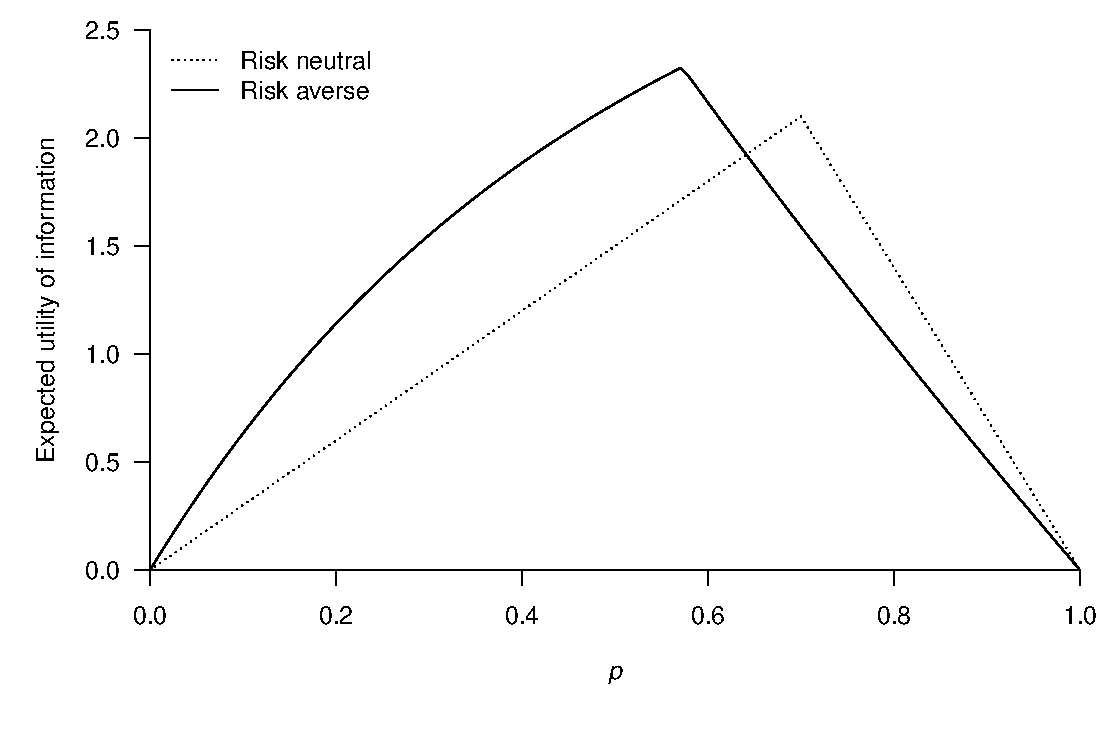
\includegraphics{_main_files/figure-latex/eupi-1.pdf}
\caption{\label{fig:eupi}The expected utility of information. Lines indicate the
relationship between the expected utility of information and probability
of restoration failing. Dotted line is for a risk-neutral decision maker
while the solid line indicates the same relationship for their
risk-averse counterpart. In both cases the expected utility of
information peaks at the critical point along the x-axis where the
optimal strategy switches from ``restore'' to ``do nothing''.}
\end{figure}

\subsection*{Conclusion}\label{conclusion}
\addcontentsline{toc}{subsection}{Conclusion}

So to reiterate, risk tolerance matters to decision making and the value
of information. Though the risk-averse are relatively intolerant to a
risk of failure, it does not automatically follow that eliminating
uncertainty with new information will be viewed more favourably to the
risk-averse than to the more risk tolerant. Sometimes in fact, the
opposite is true. Sometimes the act of seeking new information becomes
the risky decision itself and in such circumstances a risk-averse
conservation decision maker will show less preference for learning than
would a risk-neutral one. As a consequence risk profile cannot be taken
for granted when valuing information for conservation and resource
management. Careful assessment of risk tolerance is needed to know for
sure how much to invest in learning before making decisions.

\bibliography{voiRisk.bib}


\end{document}
